\chapter{Traffic modelling techniques}
\label{cha:traffic-forecasting-techniques}

In this chapter, we present the techniques we borrow from transportation research to estimate the origin-destination matrix we used in Chapter~\ref{chap:implementation} to characterize the logical links of the offloading overlay from road traffic counts. 

In our evaluations of Chapter~\ref{chap:implementation} and~\ref{cha:feasibility-study} , we used publicly available datasets with \acrfull{aadt}\index{AADT} for the road segments to estimate the road traffic volumes on the paths connecting the offloading spots. Recall that \acrshort{aadt} is the total volume of traffic traveling on a road segment in both directions for one year, divided by the number of days in the year. The traffic modelling process\index{traffic modelling techniques} follows the steps detailed in the rest of this chapter.

\section{Route determination}
\label{sec:route-determination}

\begin{wrapfigure}[13]{o}[0.4\marginparwidth]{5.5cm}
    \vspace{-10pt}\resizebox{0.9\linewidth}{!}{\begin{tikzpicture}[node distance=2cm]
	\tikzset{
	    bigN/.style={draw,circle,minimum width=0.3cm,inner sep=0},
	    smallN/.style={draw,circle,minimum width=0.3cm,inner sep=0} 
	}
	\node[bigN] (1) at (0,0) {} 
		node[smallN,fill=red] at (1.center) {}
		node at (1.south) [below] {$S$};
	\node[smallN] (3) at (1.5,0.65) {};
	\node[smallN] (2) at (2,-1) {};
	\node[smallN] (4) at (3,-0.5) {};
	\node[smallN] (5) at (3.5,0.25) {};
	\node[smallN] (6) at (4.5,-1.5) {};
	\node[smallN] (7) at (5,1) {};
	
	\node[smallN,dashed] (8)  at (6,2.5) {};
	\node[smallN,dashed] (9) at (6,-1.7) {};
	\node[smallN,dashed] (10) at (7,0.5) {};
	
	\draw (1) -- (2);
	\draw (1) -- (3);
	\draw (1) -- (4);
	\draw (1) -- (5);
	\draw[thick] (1) -- (6);
	\draw[thick] (1) -- (7);
	
	\fill[pattern=custom north west lines,hatchcolor=red] 
		  (-30:5cm) -- (-30:5.5cm)
	      arc (-30:30:5.5cm) -- (30:4.5cm)
	      arc (30:-30:4.5cm) -- cycle;
	\fill[red] 
		  (-30:5.5cm) -- (-30:6cm)
	      arc (-30:30:6cm) -- (30:5.5cm)
	      arc (30:-30:5.5cm) -- cycle;
	\draw[red] (1) -- (-30:6cm) 
		node [pos=0.82,below,sloped] {\textit{refill}};
	\draw[red] (1) -- (30:6cm)
			node [pos=0.4,above,sloped] {Range of the vehicle}
			node [pos=0.98,above,sloped] {\textit{critical}};
	\node[anchor=base west] at ($(-30:6cm) +(0:0.2cm)$) {\textit{Out-of reach}};
\end{tikzpicture}}
\vspace{-5pt}
    \caption{Illustration of the range of a vehicle and the offloading spots within its range.}
    \label{fig:vehicle-range}
\end{wrapfigure}

The first step\index{transportation modelling!route determination} consists of selecting a subset of the alternative routes connecting each pair of adjacent offloading spots in the road network. Adjacent offloading spots are those within a pre-defined range of the vehicles as shown in Figure~\ref{fig:vehicle-range}. In the case of electric vehicles, the range is limited to the autonomy of the battery. Current electric vehicles have an autonomy of 300~km on average (\eg up to 473~km for the Tesla Model S 90D\footnote{\url{https://www.Teslamotors.com/models}}, 210~km for the Renault Zoe\footnote{\url{http://www.renault.fr/gamme-renault/vehicules-electriques/zoe}}, and 180~km for the Nissan LEAF\footnote{\url{http://www.nissanusa.com/electric-cars/leaf/charging-range/}}). In the case of internal combustion engine\index{internal combustion engine} vehicles, the range is generally higher than electric vehicles. Note that the range of the vehicles highly depends on the driving behavior of the drivers. In the simulations of the following chapters, we considered a conservative vehicle range of 300~km.

The selection of the road paths consists in choosing the paths that are the most relevant to the behavior of the drivers. A natural approach to this problem is to use the All-or-Nothing assignment, which assigns the road traffic to the shortest route between two points~\cite{dijkstra1959note,delling2009engineering,hart1968formal}. While the shortest route may be used by most of the drivers, it does not account for the alternative routes chosen by other drivers, in the case of congestion or road work for instance. To determine multiple routes, on can use algorithms that compute the $k$-shortest routes in terms of travel time~\cite{yen1971finding,eppstein1998finding}. However, for large networks, these algorithms yield routes that are most of the time not reasonable and not actually used by the drivers. More recent algorithms try to determine the most reasonable alternative routes between two points~\cite{geisberger2010route,abraham2013alternative}. In the evaluations of Chapter~\ref{chap:implementation}, we use the algorithm proposed by Abraham \etal~\cite{abraham2013alternative} to determine the most reasonable alternative routes in the road network of France. With this algorithm, the routes are selected such that they share a low degree of similarity in terms of road segments in common. 

\section{Route assignment}
\label{sec:route-assignment}

The second step\index{transportation modelling!route assignment} consists in assigning weights to the selected routes. The weights give the proportion of traffic $p(k)$ that will use a certain route $k$. If only one route $k$ was selected by a shortest-path algorithm, then, all the road traffic is assigned to this route and $p(k) = 1$. However, if a set of road paths were selected in the route determination step, we determine the proportion of traffic to assign to each selected route using route choice and traffic assignment strategies. These strategies determine weights to the selected routes. The values of the weights are determined according to attributes such as the travel time and the distance of the routes. 
\begin{wrapfigure}[16]{o}[0.7\marginparwidth]{7.5cm}
    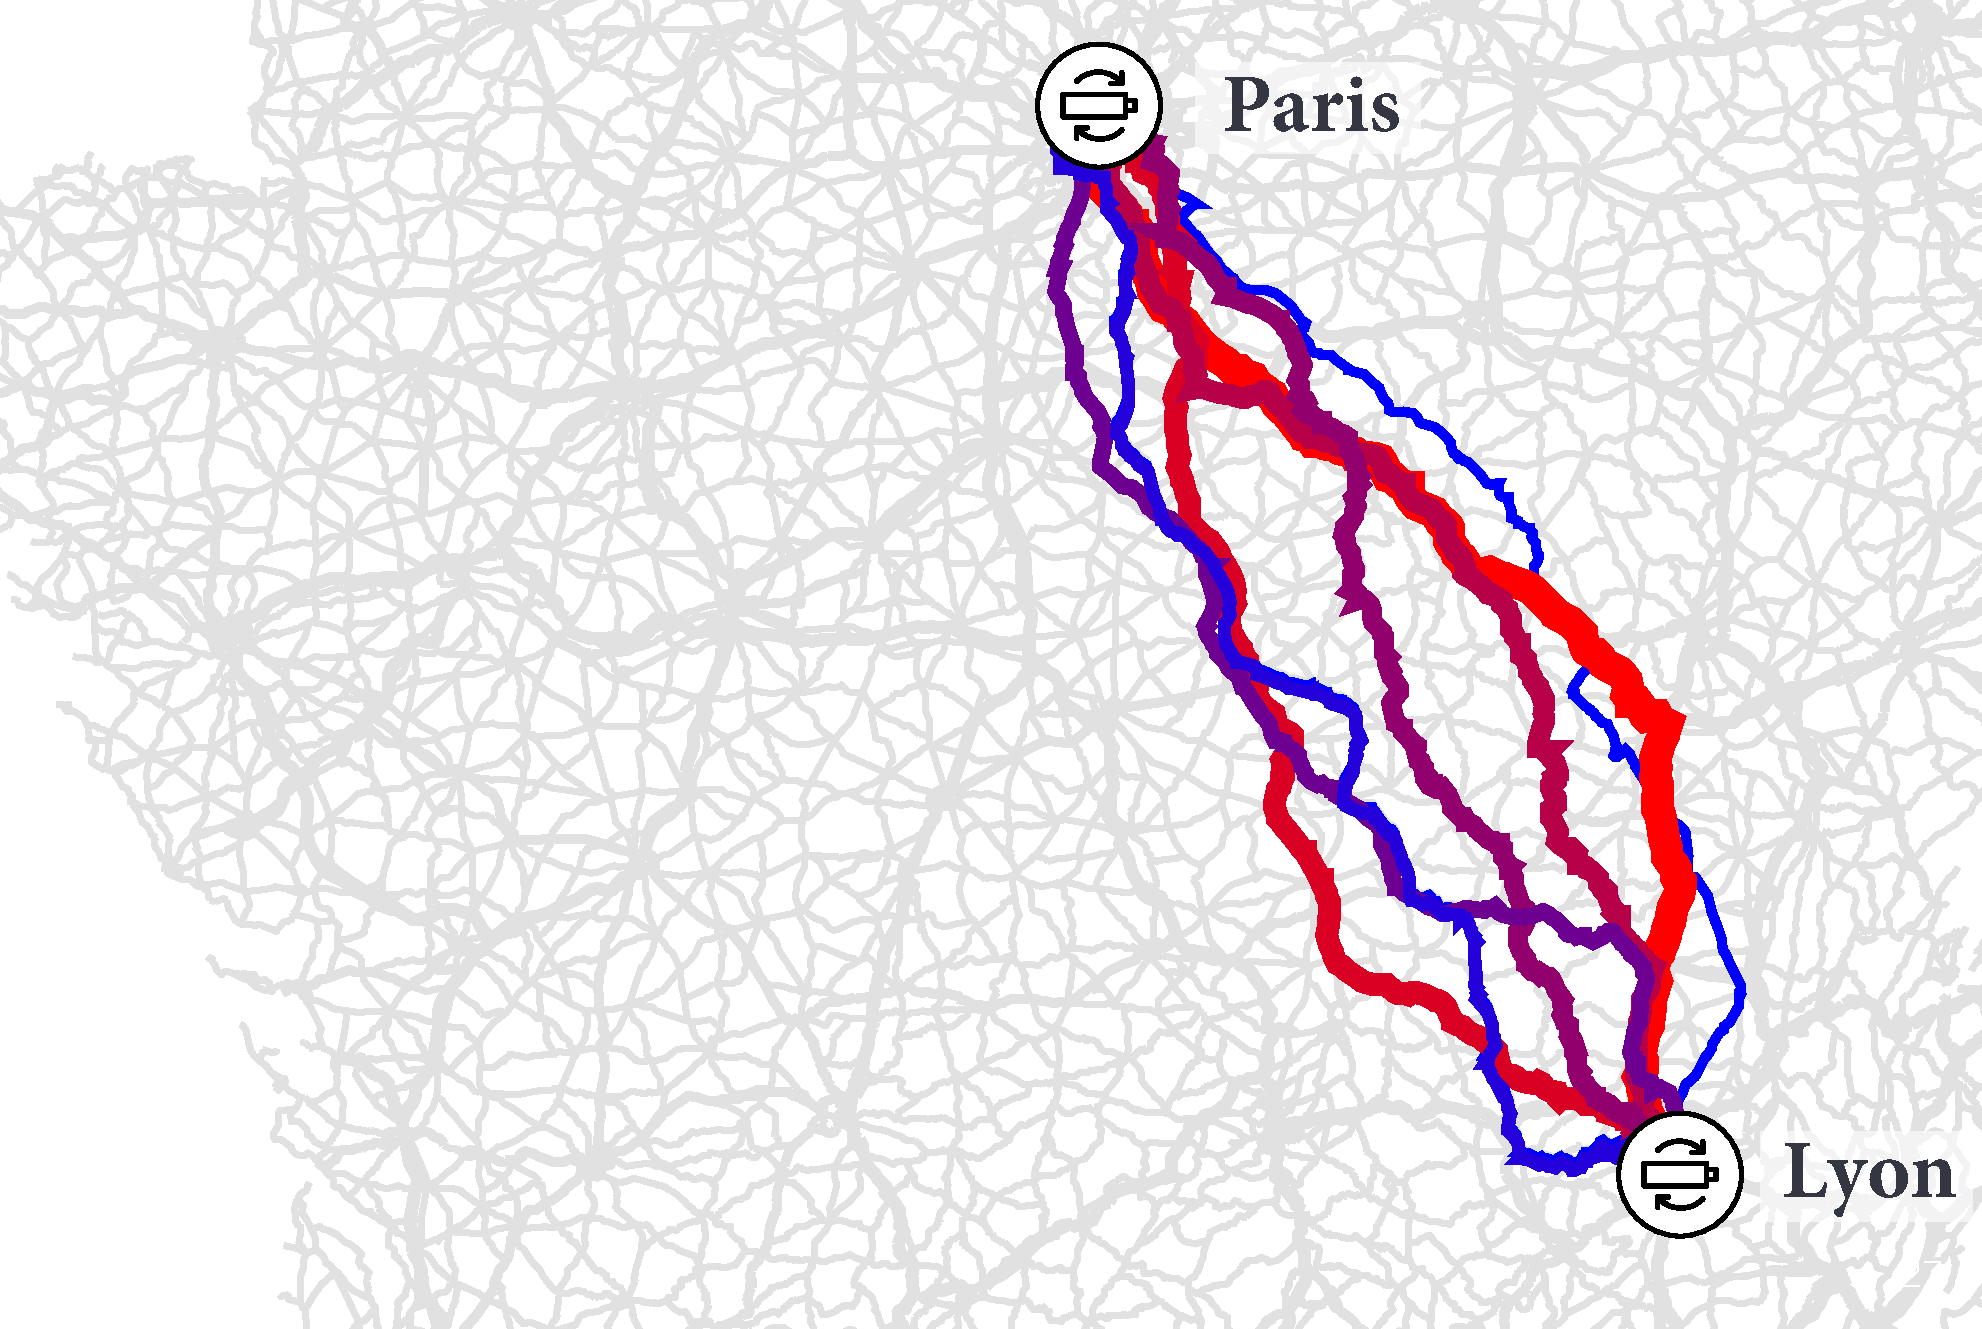
\includegraphics[width=7cm]{figures/route-assignment.pdf}
    \caption{Top 10 routes between Paris and Lyon chosen with the algorithm proposed by Abraham \textit{et al.}~\cite{abraham2013alternative}. The red thickest route is the shortest path and the width of the routes depends on the weights assigned to the routes by the C-Logit traffic assignment~\cite{cascetta1996modified}.}
    \label{fig:route-assignment}
\end{wrapfigure}
Those weights reflect the capacity of a route in attracting traffic, the higher the weight of a route, the more traffic it will receive. To this end, stochastic-user-equilibrium (S-U-E) techniques~\cite{daganzo1977stochastic} were derived from the user-equilibration criterion formulated by Wardrop~\cite{wardrop1952some}. The user-equilibration criterion specifies the following two principles:
\begin{enumerate}
    \item In an equilibrated network, users cannot improve their travel time by changing routes.
    \item The average journey time of all drivers is at a minimum.
\end{enumerate}
The S-U-E techniques build on Wardrop's principles to propose stochastic route assignment algorithms. These techniques include Dial's or C-Logit stochastic traffic assignments~\cite{dial1971probabilistic,cascetta1996modified}.  In the evaluations of Chapter~\ref{chap:implementation}, we use the C-logit route assignment model~\cite{cascetta1996modified} to determine the weights on the selected routes in the road network of France. The C-Logit traffic assignment is a multinominal logit model that assigns a choice probability $p(k)$ on a path $k$ using a perceived utility $U_k$ to each path $k$ of the selected paths:
\begin{equation}
U_k = V_k + \varepsilon_k\quad \forall k,
\end{equation}
where $V_k$ is the average or systematic utility of path $k$ (\eg distance or travel time) and $\varepsilon_k$ is the random residual that includes perception errors of the user’s decisions. Here, we consider the utility $V_k$ is the sum of the inverse of the travel time of each road segment in the road path $k$.

The choice probability, or weight, $p(k)$ for path $k$ is expressed as:
\begin{equation}
p\left(k\right)=\frac{\exp\left[V_{k}-CF_{k}\right]}{\sum_{h\in\mathcal{{P}}^{st}}\exp\left[V_{h}-CF_{h}\right]}\Comma
\end{equation}
where the term $CF_{k}$ is the ``commonality factor'' of path $k$, which is directly proportional to the degree of similarity of path $k$ with the other selected paths. Here, we consider the following expression of the commonality factor:
\begin{equation}
CF_{k}=\beta_{0}\ln\sum_{h\in\mathcal{P}^{st}}\left(\frac{L_{hk}}{L_{k}^{1/2}L_{h}^{1/2}}\right)^{\gamma}\Comma
\end{equation}
where $L_{hk}$ is the length of common paths to $h$ and $k$, $L_{h}$ and $L_{k}$ are the lengths of paths $h$ and $k$, respectively, and $\gamma$ is a positive parameter. Typically, $\beta_{0} = 1$ and $\gamma = 1$ or $\gamma = 2$~\cite{cascetta1996modified}.

The weights determined by the traffic assignment techniques are then used in combination with the traffic counts to estimate the traffic volume of the routes selected in the first step between each pair of adjacent offloading spots. 


\section{Trip matrix estimation}
\label{sec:trip-matrix-estimation}

Finally, in the third step\index{transportation modelling!trip matrix estimation}, we determine the origin-destination trip matrix that characterizes the number of trips between each pair of adjacent offloading spots. This step can be done qualitatively by conducting travel surveys to know the travel habits of the populations within a geographical area. Examples of these national surveys include the \acrfull{nhts} in the United States\footnote{\url{http://nhts.ornl.gov}} and the \acrfull{entd} in France.\footnote{\url{http://www.statistiques.developpement-durable.gouv.fr/sources-methodes/enquete-nomenclature/1543/139/enquete-nationale-transports-deplacements-entd-2008.html} (in French)} These surveys are conducted by governmental agencies about every ten years. The last version of the \acrshort{nhts} dates from 2009 while the last version of the \acrshort{entd} dates from 2008. There is currently a newer version (2016) of the \acrshort{nhts} survey being conducted. A lower bound of an estimate of the road traffic $T_{ij}$ between pairs of locations $(i,\,j)$ corresponds to the traffic volume $v_{ab}$ of the road segment $(a,\,b)\in L^{R}$ with the lowest traffic of the shortest road path $k$ between the two locations (\ie that corresponds to the bottleneck of the road path). The volume is weighted by $w(d(k))$, the proportion of trips accounted in travel surveys of the same distance as the one of the shortest road path $d(k)$. This estimate can be expressed as follows:
\begin{equation}
    T_{ij} = w(d(k))\times\min_{(a,\,b)\in k}\{v_{ab}\},
\end{equation}

Because these surveys take time and are expensive to conduct, there exist other techniques to estimate traffic matrices between selected locations. These techniques usually rely on \acrfull{aadt}\index{AADT}. It is important to underline that the \acrshort{aadt} is a fundamental statistic used in traffic engineering and transportation planning. The use of the \acrshort{aadt} helps reduce the effects of seasonal bias and missing data mainly due to equipment failure, construction schedules, and installation dates that plague continuous traffic monitoring~\cite{wright1997variability}.

In particular, Zuylen and Willumsen~\cite{van1980most} proposed an entropy-maximizing formulation\index{entropy-maximization problem|bb} to estimate the most likely \acrfull{od} trip matrix\index{origin-destination trip matrix|bb} between the defined locations. The objective of the formulation is to maximize the number of ways of selecting an \acrshort{od} matrix with a total number of trips. As the number of trips increases, the number of ways of selecting an \acrshort{od}  matrix gets more and more peaked and converges to a most likely state. This results in maximizing the entropy of the \acrshort{od}  matrix. The constraint guarantees that the resulting \acrshort{od}  matrix will not overcome the volumes of traffic $v_a$ measured on the road segments $a$. 
\begin{flalign*}
    & \text{Maximize} -\sum_{ij}\big(T_{ij}\log T_{ij} - T_{ij}\big), & \\
    \shortintertext{subject to}
    & v_{a} - \sum_{ij}T_{ij}p^{a}_{ij} = 0 \qquad \forall a \in L^{R}.\\
\end{flalign*}
The probability $p^{a}_{ij}$ denotes the route choice probability of route between source $i$ and destination $j$ to take link $a$ among $S_{ij}$, the set of selected road path. This probability is derived from the choice probability and computed in the route assignment as follows:
\begin{equation}
p^{a}_{ij} = \sum_{\substack{k\in S_{ij}\\k\ni a}} p(k),
\end{equation}

\begin{algorithm}
    \caption{Iterative balancing algorithm for the entropy maximization problem.}
	\DontPrintSemicolon
	\SetKwBlock{Step}{}{}
		
	\Step(\textbf{Step 1.} Initialization){
		$\lambda_{a} \gets 0\quad \forall a\in L$\;
	}	
		
	\BlankLine
	
	\Step(\textbf{Step 2.} Iterative balancing){
		\Repeat{Convergence}{
			$T_{ij}^{\star} \gets \exp\left(\sum_{a}\lambda_{a} \, p^{a}_{ij}\right)\quad \forall i,\,j$\;
			\ForAll{constraints (over domain $L^{R}$)}{
				\If{$V_{a} \neq \sum_{ij}T_{ij}^{\star} \, p^{a}_{ij} $}{
					$\lambda_{a} \gets \lambda_{a} + \ln(V_{a}) - \ln\left(\sum_{ij}T_{ij}^{\star} \, p^{a}_{ij}\right)$
				}
			}
		}
	}
    \label{alg:iterative-balancing}
\end{algorithm}


Since the optimization problem presented above is convex, the authors presented an iterative balancing algorithm to solve it, derive from Bergman's method to solve such problems~\cite{bregman1967proof}. The algorithm is presented in Algorithm~\ref{alg:iterative-balancing}. Each balancing iteration adjusts the quantity $\lambda_{a}$, the road traffic assigned to each road segment $a$. This adjustment is done until all the constraints on the volumes of the road segments are satisfied.

With the traffic modelling techniques presented in this appendix, we were able to derive the traffic volumes on the road paths connecting the offloading spots from traffic counts on road segments. In the vehicle flow allocation problem of Chapter~\ref{chap:implementation}, we used these traffic volumes to characterize the logical links of the offloading overlay that connect offloading spots together.